\chapter{Experiments and results}

\section{Preamble}
This chapter provides information on all the various experiments conducted with their parameters, figures and tables, and the conclusion derived from these experiments. 

\section{Experiment design}

\begin{table}
\centering
\caption{Default Parameters}
    \begin{tabular}{||c c||}
    \hline
    {\bf Parameters}     & {\bf Value} \\ \hline

  	PU Active Probability 	& $P(H_1)=0.5$	\\ \hline
  	Bandwidth 			& $w=5  MHz$	\\ \hline
  	Sampling Frequency 	& $\tau=10MHz	$	\\ \hline
  	Number of Samples	& $K=2\tau w= 50$		\\ \hline
  	Number of SUs 		& $S=3$		\\ \hline
	SU distance from PU  	& [500,750,1000]	\\ \hline
  	Training Dataset Size 	& 250		\\ \hline
  	Testing Dataset Size 	& 50000		\\ \hline
  	Fading Scenario		& Rayleigh		\\ \hline
	Fading Variance		& 2			\\ \hline
    \end{tabular}
\end{table} 


Here various experiments are conducted showing performance of Spectrum Sensing, they are as follows:
\begin{itemize}
\item Performance of All Algorithms
\item Performance of Spectrum Sensing under various Fading Scenarios
\item Performance with respect to varying Sensing Time
\item Performance with respect to varying SU numbers
\item Performance of MAchine Learning algorithms with respect to varying Training Dataset Size \\
\end{itemize}





\subsection{Experiment 1: Performance of All Algorithms}
\begin{table}
\centering
\caption{AUC Values for all algorithms}
    \begin{tabular}{||c c c c c||}
    \hline
    {\bf Algorithms} & {\bf Rayleigh} & {\bf Rayleigh} & {\bf Rician} & {\bf Rician} \\ \hline
    - &  Var=1 &    Var=2 &   Var=1 & Var=2  	\\ \hline

       	Linear SVM 	& 0.8646	& 0.9376	& 0.9041	& 0.9677	\\ \hline
  	Logistic 		& 0.8642	& 0.9373	& 0.9043	& 0.9661	\\ \hline
  	MLP 			& 0.8622	& 0.9376	& 0.9059	& 0.9632	\\ \hline
  	Gaussian SVM 	& 0.8624	& 0.9353	& 0.9038	& 0.9680	\\ \hline
  	OR 			& 0.8434	& 0.9258	& 0.8787	& 0.9579	\\ \hline
  	MRC  			& 0.8571	& 0.9252	& 0.9020	& 0.9631	\\ \hline
  	Naive Bayes 	& 0.8459	& 0.9250	& 0.8909	& 0.9637	\\ \hline
  	XGBoost 		& 0.8349	& 0.9142	& 0.8926	& 0.9645	\\ \hline
  	CatBoost 		& 0.8474	& 0.9218	& 0.8856	& 0.9622	\\ \hline
  	ADABoost 		& 0.8376	& 0.9203	& 0.8816	& 0.9594	\\ \hline
  	RandomForest 	& 0.8320	& 0.9195	& 0.8762	& 0.9598	\\ \hline
  	KNN 			& 0.8407	& 0.9109	& 0.8859	& 0.9610	\\ \hline
  	S1 			& 0.8437	& 0.9092	& 0.8924	& 0.9552	\\ \hline
  	S2 			& 0.6453	& 0.7275	& 0.6548	& 0.7571	\\ \hline
  	AND 			& 0.6718	& 0.7357	& 0.6919	& 0.7642	\\ \hline
	S3 			& 0.5546	& 0.6001	& 0.5524	& 0.6044	\\ \hline
    \end{tabular}
\end{table} 




\begin{table}
\centering
\caption{AUC Values for all algorithms}
    \begin{tabular}{||c c c c c c||}
    \hline
    {\bf Algorithms} & {\bf Nakagami} & {\bf Nakagami} & {\bf Nakagami} & {\bf Nakagami} & {\bf AWGN} 			\\ \hline
    -  & Var=1 M=0.5& Var=1 M=1& Var=1 M=1.5& Var=1 M=2& - 	\\ \hline

    	Linear SVM 	& 0.8114	& 0.8592	& 0.8871	& 0.9042	& 0.9618	\\ \hline
  	Logistic 		& 0.8094	& 0.8613	& 0.8753	& 0.9039	& 0.9580	\\ \hline
  	MLP 			& 0.7880	& 0.8618	& 0.8843	& 0.8996	& 0.9611	\\ \hline
  	Gaussian SVM 	& 0.8110	& 0.8619	& 0.8896	& 0.8937	& 0.9617	\\ \hline
  	OR 			& 0.8006	& 0.8436	& 0.8619	& 0.8756	& 0.9295	\\ \hline
  	MRC  			& 0.7977	& 0.8577	& 0.8856	& 0.9016	& 0.9618 	\\ \hline
  	Naive Bayes 	& 0.7970	& 0.8477	& 0.8778	& 0.8927	& 0.9600	\\ \hline
  	XGBoost 		& 0.7945	& 0.8361	& 0.8457	& 0.8919	& 0.9395	\\ \hline
  	CatBoost 		& 0.7794	& 0.8484	& 0.8668	& 0.8772	& 0.9503	\\ \hline
  	ADABoost 		& 0.7878	& 0.8492	& 0.8683	& 0.8801	& 0.9427	\\ \hline
  	RandomForest 	& 0.7655	& 0.8413	& 0.8607	& 0.8495	& 0.9377	\\ \hline
  	KNN 			& 0.7741	& 0.8227	& 0.8728	& 0.8727	& 0.9444	\\ \hline
  	S1 			& 0.7812	& 0.8448	& 0.8753	& 0.8923	& 0.9580	\\ \hline
  	S2 			& 0.6247	& 0.6453	& 0.6474	& 0 .6502	& 0.6617	\\ \hline
  	AND 			& 0.6401	& 0.6704	& 0.6824	& 0.6905	& 0.7108	\\ \hline
	S3 			& 0.5531	& 0.5526	& 0.5474	& 0.5524	& 0.5522	\\ \hline
    \end{tabular}
\end{table} 


\begin{figure}
  \begin{center}
  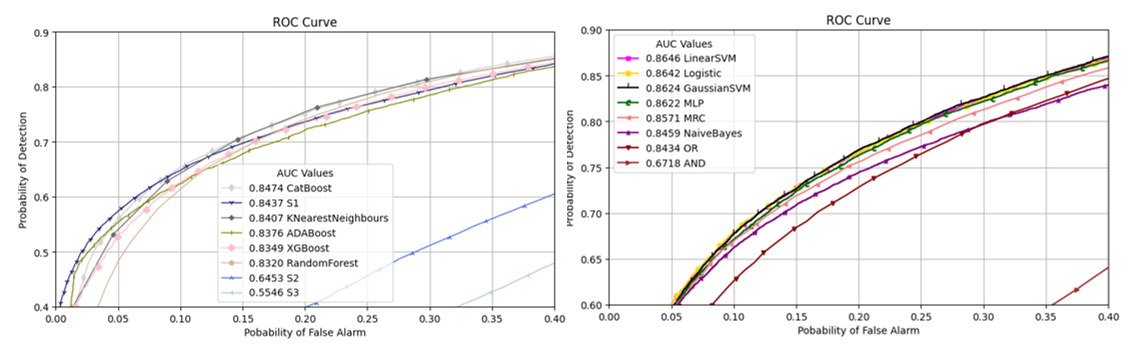
\includegraphics[width=1\textwidth]{figs/2.png}
  \end{center}
  \caption{ROC Curves for Rayleigh Fading Variance=1}
\end{figure}

\begin{figure}
  \begin{center}
  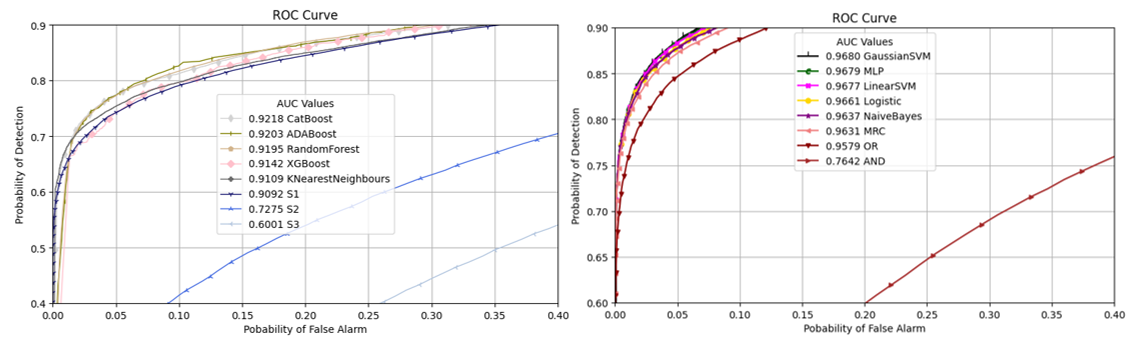
\includegraphics[width=1\textwidth]{figs/3.png}
  \end{center}
  \caption{ROC Curves for Rayleigh Fading Variance=2}
\end{figure}

\begin{figure}
  \begin{center}
  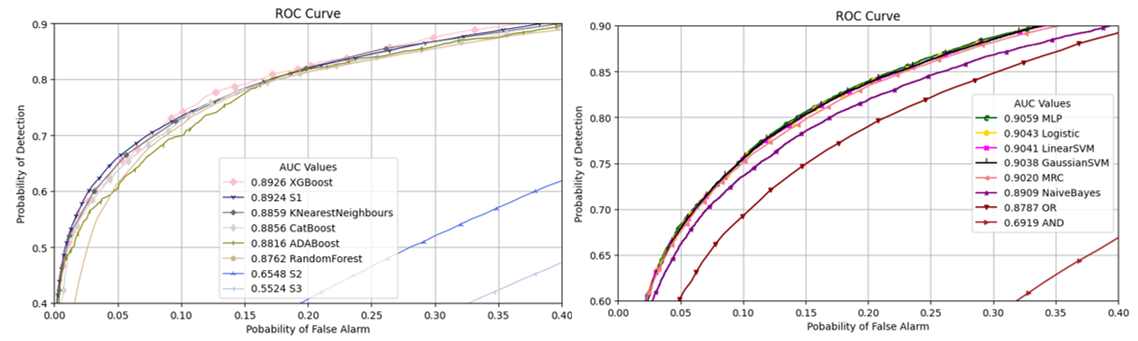
\includegraphics[width=1\textwidth]{figs/4.png}
  \end{center}
  \caption{ROC Curves for Rician Fading Variance=1}
\end{figure}

\begin{figure}
  \begin{center}
  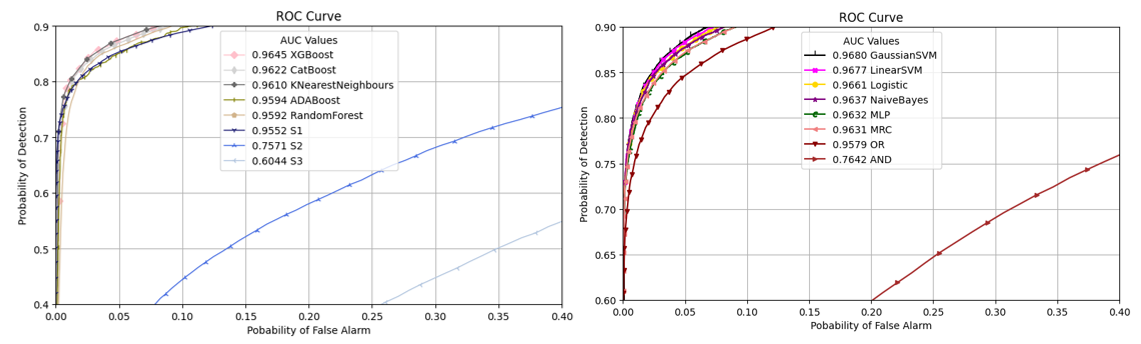
\includegraphics[width=1\textwidth]{figs/5.png}
  \end{center}
  \caption{ROC Curves for Rician Fading Variance=2}
\end{figure}

\begin{figure}
  \begin{center}
  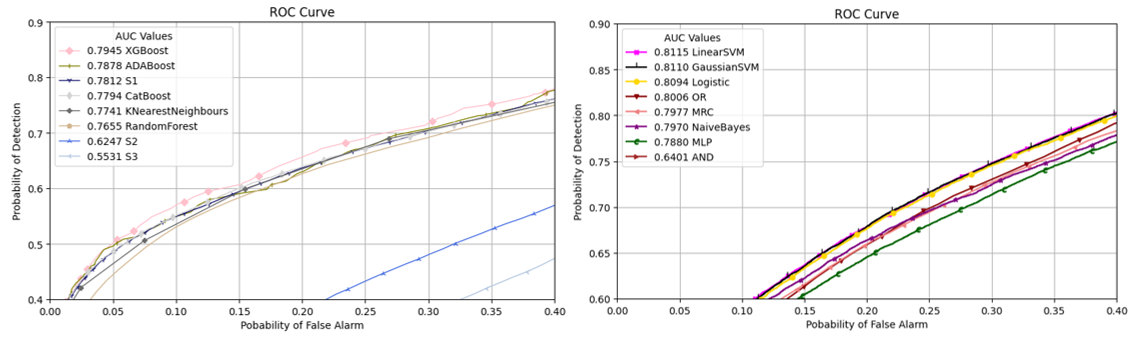
\includegraphics[width=1\textwidth]{figs/6.png}
  \end{center}
  \caption{ROC Curves for Nakagami Fading Variance=1 M=0.5}
\end{figure}

\begin{figure}
  \begin{center}
  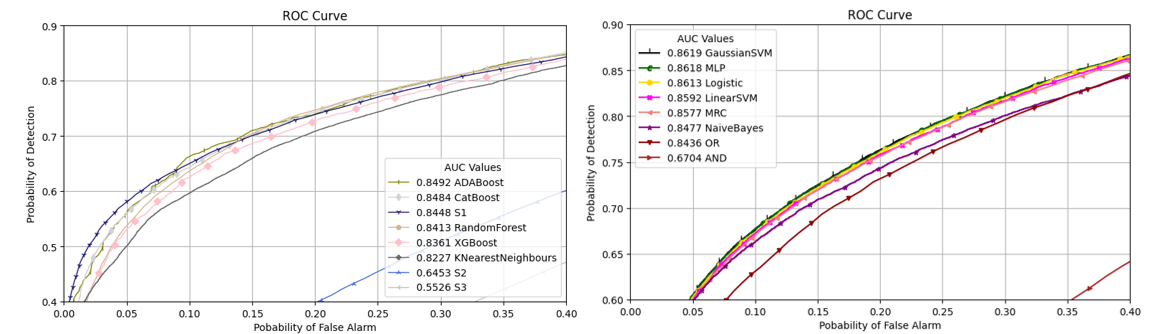
\includegraphics[width=1\textwidth]{figs/7.png}
  \end{center}
  \caption{ROC Curves for Nakagami Fading Variance=1 M=1}
\end{figure}

\begin{figure}
  \begin{center}
  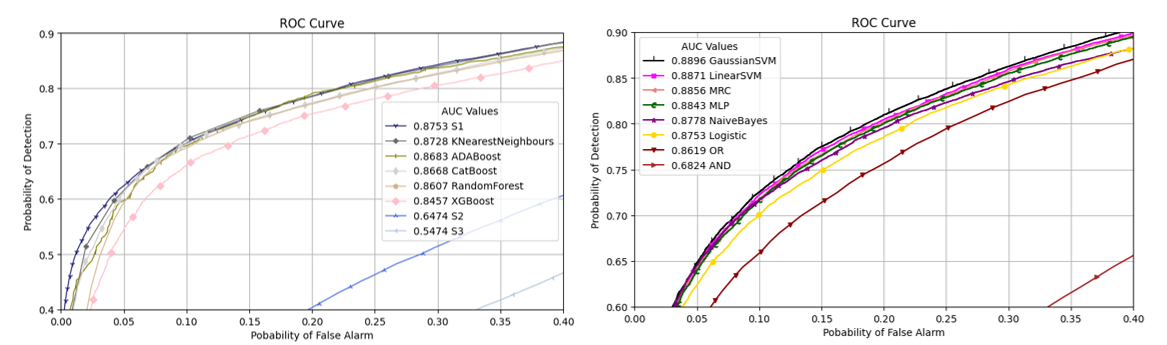
\includegraphics[width=1\textwidth]{figs/8.png}
  \end{center}
  \caption{ROC Curves for Nakagami Fading Variance=1 M=1.5}
\end{figure}

\begin{figure}
  \begin{center}
  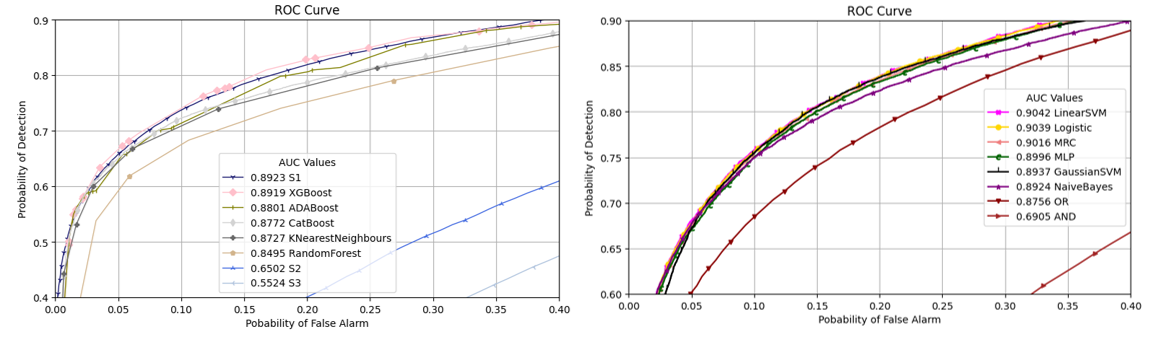
\includegraphics[width=1\textwidth]{figs/9.png}
  \end{center}
  \caption{ROC Curves for Nakagami Fading Variance=1 M=2}
\end{figure}

\begin{figure}
  \begin{center}
  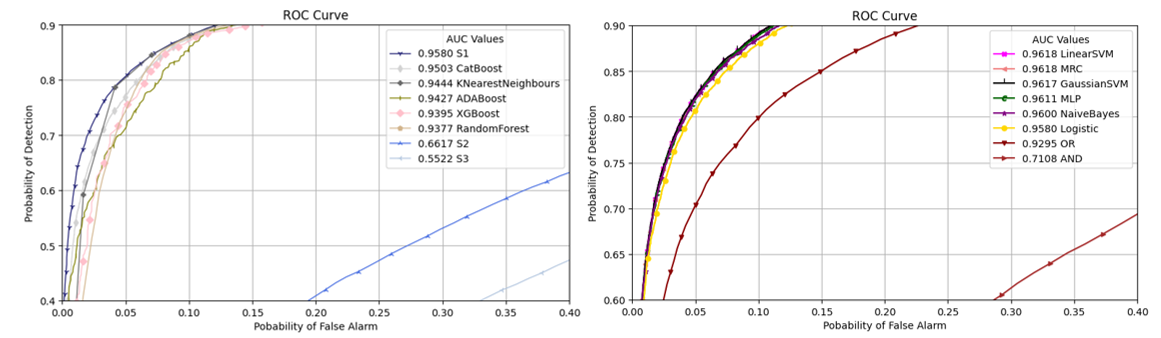
\includegraphics[width=1\textwidth]{figs/10.png}
  \end{center}
  \caption{ROC Curves for AWGN}
\end{figure}

\subsubsection{Parameter settings}
AUC Values for all algorithms has been compared with fading scenarios for 250 training dataset size, 50000 test dataset, $\tau=5\mu s$ ($K=50$ Samples) for $SU=3$. Various Non-cooperative techniques, Classical Cooperative Techniques, and Machine Learning Techniques have been used for various fading scenarios.

Fig. 4.1-4.9 (a) contains S1, S2, S3 (Non-cooperative Algorithm for each SU), XGBoost, CatBoost, ADABoost, Random Forest Classifier, and K Nearest Neighbours.

Fig. 4.1-4.9 (b) contains Logistic Regression, Linear SVM, Gaussian SVM, MLP, Naive Bayes, and AND, OR, MRC (Classical Cooperative Spectrum Sensing Techniques).
\subsubsection{Results and discussion}
With reference to Fig. 4.1-4.9, 4.10 and Table 4.2 and 4.3, talking about Non-cooperative Spectrum Sensing algorithms first, they rank last in performance. Only S1 has acceptable performance, as it is closest to the PU. Perforamance of S3 is only a little better than a random coin flip. The closer an SU is to the PU, the better its performance is. For classical algorithms, AND is the worst performing algorithm of the three. This is because, even if one SU decides that the PU is not transmitting, the final decision is that the PU is not actively using the spectrum which leads to a lot of false alarms. OR gives much better performance because it minimises false alarms, all SUs have to agree that the PU is not transmitting. MRC comes out at the top, with OR method not far behind. This is because MRC is the only algorithm in the test suite that has knowledge of SNR values and it accordingly decides how much priority should be given to each SU in terms of their decision. 
Coming to Decision Tree based algorithms, they do not have the best performance, but the boosting gradient algorithms consistently outperform Random Forest Classification, proving that they do have potential. K Nearest Neighbours and Naïve Bayes are simpler algorithms and not very robust, hence they hardly outperform powerful algorithms like MLP. In Machine Learning algorithms, the top 4 algorithms are Linear SVM, Gaussian SVM, MLP and Logistic Regression. SVMs are powerful they focus at samples from one label that are closer to the other label (worst case samples). Logistic Regression is simple and robust. MLP does not clearly come at the top, because it is limited by the training dataset size and it only has one hidden layer, yet all four algorithms (Fig. 4.10) are very close in terms of performance, and there is no clear winner, and all four Machine Learning algorithms are suitable, and they consistently outperform Classical Algorithms.


\subsection{Experiment 2: Performance of All Fading Scenarios}
\begin{figure}
  \begin{center}
  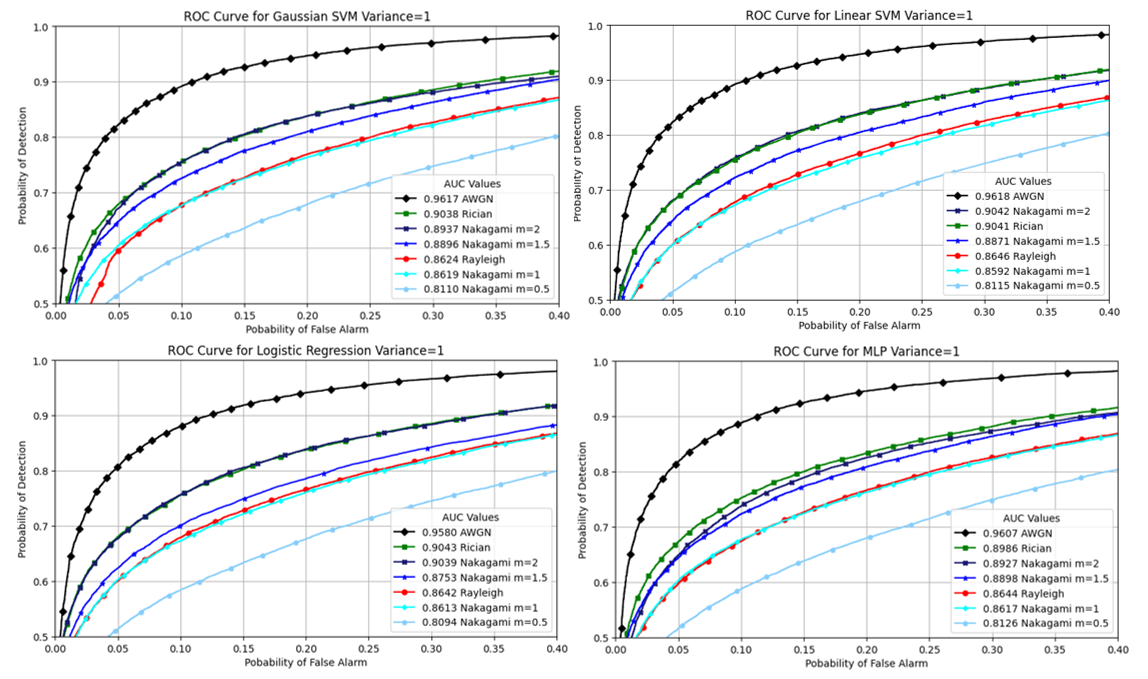
\includegraphics[width=1\textwidth]{figs/1.png}
  \end{center}
  \caption{ROC Curves depicting performance of ML Algorithms for All Fading Scenarios}
\end{figure}

\subsubsection{Parameter settings}
AUC Values for all algorithms has been compared with fading scenarios for 250 training dataset size, 50000 test dataset, $\tau=5\mu s$ ($K=50$ Samples) for $SU=3$ (4.1.1).

AUC Values for Gaussian SVM, Linear SVM, MLP and Logistic Regression have been compared fading scenarios for 250 training dataset size, $\tau=5\mu s$ ($K=50$ Samples) for $SU=3$. Curves for Rayleigh Fading, Rician Fading, Nakagami Fading, and AWGN have been plotted for each algorithm at $Variance=1$.
\subsubsection{Results and discussion}
With respect to Fig 4.10, Rayleigh Fading (Fig. 4.1 and 4.2) performs the worst, as it assumes that there is no line-of-sight communication, but is the most practical scenario in urban areas. Rician fading (Fig. 4.3 and 4.4) scenario algorithms outperform Rayleigh Fading algorithms because there is line-of-sight communication, so there is a clearer difference in the energy values for H1 and H0. Increasing the M (shape) parameter, for Nakagami Fading (Fig. 4.5-4.8) reduces the effect of fading, which in turn increases the performance. AWGN (Fig. 4.9) outperforms all other fading scenarios, because there is no fading present and this scenario generates the simplest data for algorithms. Fig. 4.10 compares performance of the four best algorithms under all fading scenarios. Rayleigh Fading and Nakagami Fading with parameter M=1 (which is Rayleigh Fading) only have a small difference which can come down to the small variations in the dataset. The difference is larger in MLP only because MLP learns differently and the weighs are different every time, all algorithms have trained on the same dataset corresponding to a fading scenario. Variance=2 (Fig. 4.2, 4.4) is a better scenario compared to Variance=1 (Fig. 4.3, 4.5) because now the random sample has a higher magnitude, and the gain is multiplied with the signal, hence the energy values for H1 are higher, making it easier to differentiate between the two labels.

\subsection{Experiment 3: Verying Sensing Time}

\begin{figure}
  \begin{center}
  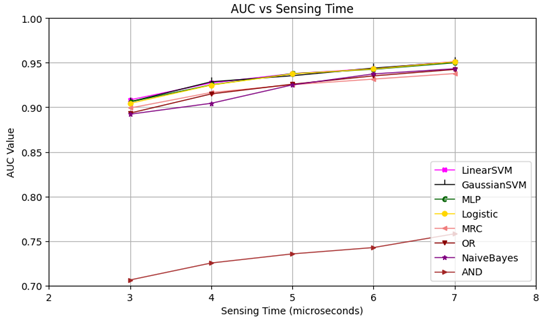
\includegraphics[width=0.9\textwidth]{figs/11.png}
  \end{center}
  \caption{AUC vs Sensing Time}
\end{figure}

\subsubsection{Parameter settings}

Here $\tau$ ranges from $[3\mu s,7\mu s]$ and hence K ranges from [30,70] samples (Figure 11), using Linear SVM, Gaussian SVM, MLP, Logistic Regression, Naïve Bayes, AND, OR, MRC algorithms. Rayleigh Fading has been used at $Variance=2$, 250 training dataset size, 50000 test dataset, for $SU=3$.


\subsubsection{Results and discussion}
With respect to Fig 4.11, an average increase of almost 0.01 is seen for every increase in $1 \mu s$ (10 Samples), and this value is higher when the number of samples is low, and slowly starts decreasing as we get closer to AUC value 1. The longer we sense, the more information we have to decide, and the clarity between energy values corresponding to the two labels increase. The performance at 70 samples with Rayleigh Fading with $Variance=2$ is comparable to AWGN performance. We can’t keep increasing the Sensing Time because that is time we could have otherwise used to transmit if the spectrum was not being used by the PU. The relationship isn’t linear, so we will reach a threshold, which is above 0.95, after which increasing the Sensing Time will not give a substantial increase in performance.

\subsection{Experiment 4: Varying numbers of SUs}

\begin{figure}
  \begin{center}
  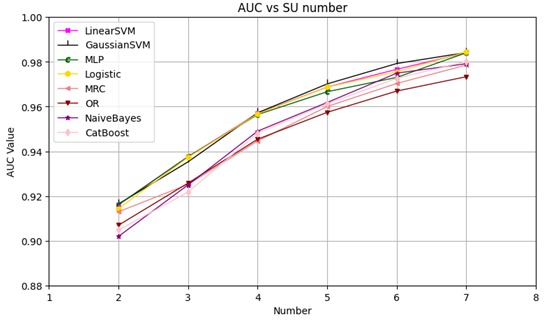
\includegraphics[width=0.9\textwidth]{figs/12.png}
  \end{center}
  \caption{AUC vs SU Numbers}
\end{figure}



\begin{table}
\centering
\caption{AUC Values with varying number of SUs }
    \begin{tabular}{||c c c c c c c||}
    \hline
    {\bf Algorithms} & {\bf 2} & {\bf 3} & {\bf 4} & {\bf 5} & {\bf 6} & {\bf 6} 			\\ \hline
    
    	Linear SVM 	& 0.9161	& 0.9376	& 0.9569	& 0.9687	& 0.9766	& 0.9840	\\ \hline
  	Logistic 		& 0.9144	& 0.9373	& 0.9567	& 0.9687	& 0.9755	& 0.9844	\\ \hline
  	MLP 			& 0.9162	& 0.9376	& 0.9564	& 0.9666	& 0.9730	& 0.9840	\\ \hline
  	Gaussian SVM 	& 0.9165	& 0.9353	& 0.9572	& 0.9701	& 0.9792	& 0.9841	\\ \hline
  	OR 			& 0.9070	& 0.9258	& 0.9454	& 0.9574	& 0.9669	& 0.9733	\\ \hline
  	MRC  			& 0.9130	& 0.9252	& 0.9446	& 0.9600	& 0.9703	& 0.9785	\\ \hline
  	Naive Bayes 	& 0.9020	& 0.9250	& 0.9490	& 0.9618	& 0.9749	& 0.9791	\\ \hline
  	XGBoost 		& 0.8957	& 0.9142	& 0.9462	& 0.9522	& 0.9689	& 0.9760	\\ \hline
  	CatBoost 		& 0.9048	& 0.9218	& 0.9481	& 0.9612	& 0.9726	& 0.9801	\\ \hline
  	ADABoost 		& 0.8938	& 0.9203	& 0.9437	& 0.9575	& 0.9691	& 0.9766	\\ \hline
  	RandomForest 	& 0.8954	& 0.9195	& 0.9450	& 0.9615	& 0.9710	& 0.9800	\\ \hline
  	KNN 			& 0.8965	& 0.9109	& 0.9430	& 0.9519	& 0.9696	& 0.9683	\\ \hline
  	AND 			& 0.7319	& 0.7357	& 0.7387	& 0.7461	& 0.7454	& 0.7486	\\ \hline
	\end{tabular}
\end{table} 

\subsubsection{Parameter settings}
Experiment implements Linear SVM, Gaussian SVM, MLP, Logistic Regression, Naïve Bayes, CatBoost, OR, MRC for Rayleigh Fading $Variance=1$. SU range is [2,7] and SUs are distributed evenly between [500m, 1000m]) in the environment from the PU. 250 training dataset size, 50000 test dataset, $\tau=5 \mu s$ ($K=50$ Samples)
\subsubsection{Results and discussion}

With respect to Fig 4.12 and Table 4.4,  The AUC value increases along with increase in SU numbers as there is more sensing data to know whether the PU is active or not. The figure shows that Cooperative Spectrum Sensing provides superior performance, and this increase in performance is highest when the number of SUs is low (for an algorithm, difference in performance of 2 SUs sensing vs 3SUs sensing is substantial), and the difference keeps decreasing as we keep on adding SUs (for an algorithm, difference in performance of 6 SUs sensing vs 7 SUs sensing is negligible).


\subsection{Experiment 5: Varying Training Dataset Size}

\begin{table}
\centering
\caption{AUC Values for all ML algorithms}
    \begin{tabular}{||c c c c c c ||}
    \hline
    {\bf Algorithms} & {\bf 50} & {\bf 100} & {\bf 250} & {\bf 500} & {\bf 1000}\\ \hline
    
    	Linear SVM 	& 0.9366	& 0.9344	& 0.9376	& 0.9360	& 0.9367	\\ \hline
  	Logistic 		& 0.9343	& 0.9344	& 0.9373	& 0.9305	& 0.9373	\\ \hline
  	MLP 			& 0.9201	& 0.9322	& 0.9376	& 0.9365	& 0.9374	\\ \hline
  	Gaussian SVM 	& 0.9378	& 0.9264	& 0.9353	& 0.9323	& 0.9368	\\ \hline
  	Naive Bayes 	& 0.9287	& 0.9152	& 0.9250	& 0.9250	& 0.9261	\\ \hline
  	XGBoost 		& 0.9192	& 0.9150	& 0.9142	& 0.9042	& 0.9274	\\ \hline
  	CatBoost 		& 0.9240	& 0.9124	& 0.9218	& 0.9213	& 0.9304	\\ \hline
  	ADABoost 		& 0.8931	& 0.9024	& 0.9203	& 0.9137	& 0.9280	\\ \hline
  	RandomForest 	& 0.9173	& 0.9020	& 0.9195	& 0.9061	& 0.9222	\\ \hline
  	KNN 			& 0.9288	& 0.9097	& 0.9109	& 0.9004	& 0.9228	\\ \hline
	\end{tabular}
\end{table} 

\subsubsection{Parameter settings}
AUC Values for all algorithms has been compared with fading scenarios for training dataset size range [50,100,250,500,1000] on the same 50000 testing dataset, $\tau=5\mu s$ ($K=50$ Samples) for $SU=3$.

\subsubsection{Results and discussion}
With reference to Table 4.5, training dataset size varies. Comparing performance of Machine Learning Algorithms. Increasing dataset size does not favour, and performance after training on 50 samples is similar to performance after training for 1000 samples. Only MLP responds to the increasing dataset size, only in the beginning, showing minor improvement. Overall, Increasing or decreasing the dataset does not affect the performance of Machine Learning algorithms, but MLP would not be a less suitable algorithm in a scenario where the machines need to train on less data or where they need to learn quickly.

\section{Overall conclusion}
We have successfully derived results and shown how the performance varies by changing various parameters, we also have found out the best algorithms for Spectrum Sensing. The results depict the order of various fading scenarios based on their performance .The code enables us to create datasets of whatever enviornment using the various parameters and fading scenarios, and we may choose any algorithm for the task of Spectrum Sensing, and we are not limited to the specific parameter values used in the experiments.

With respect to Experiment 1, Gaussian SVM, Linear SVM, MLP and Logistic Regression are the best perfroming algorithms., Graient Boosting Algorithms do not come at the top, but they do outperform Random Forest Classification consistently. For Classical algorithms, MRC is the best performing algorithm, with OR technique not far behind.

With respect to Experiment 2, We obtain best performance in AWGN scenario, as the data is much simpler to learn, followed by Rician Fading and Nakagami Fading depending upon the $M$ value, and then algorithms perform worst in Rayleigh fading scenario. Higher the variance of the Fading, bettwe is the performance.  

With respect to Experiment 3, Performance increases with increase in Sensing Time, but the increase starts to flatten as we keep increasing the Sensing Time. 

With respect to Experiment 4, Increasing the SU number increases the performance of Spectrum Sensing, the increase in performance starts flattening as we keep on increasing the SU number, and we see a substantial gain in performance  when the number of SUs are less.

With respect to Experiment 5, Varying Dataset Size does not give an increase in performance, and most algorithms will perform well even after training on 50 samples.

